\documentclass[compress]{beamer}
\usepackage[beamer, ]{ahsan}
\usepackage{listings}
\usepackage{graphicx}

\title{Percolation}
\subtitle{A powerful tool in simulation}
\author{Ipshita Bonhi}
\date{\today}

\newcommand{\imp}[1]{\textcolor{NordRed}{#1}}
\lstset{
    numbers=left,
    xleftmargin=10pt,
    numbersep=8pt,
    numberstyle=\footnotesize\ttfamily\color{fgC!60},
    stepnumber=1,
    basicstyle=\linespread{1.1}\footnotesize\ttfamily,
    commentstyle=\color{fgC!60!pageC}\ttfamily,
    stringstyle=\small\color{NordBrightBlue},
    showstringspaces=false,
    breaklines=true,
    keywordstyle=\color{NordRed},
    morekeywords={def},
    emph={[2]return, plt, as, np},
    emphstyle={[2]\color{NordOrange}},
    emph={[3]imshow, show, rand},
    emphstyle={[3]\color{NordGreen}},
}

\begin{document}

\begin{frame}[plain,noframenumbering]
    \maketitle
\end{frame}

\color{NordBlack}

\section{What is it?}


\begin{frame}
    Consider a sponge as scene at the right. This kind of medium have tiny pores
    inside a solid skeleton. These kind of mediums are called ``Porous Medium''.

    \begin{center}
        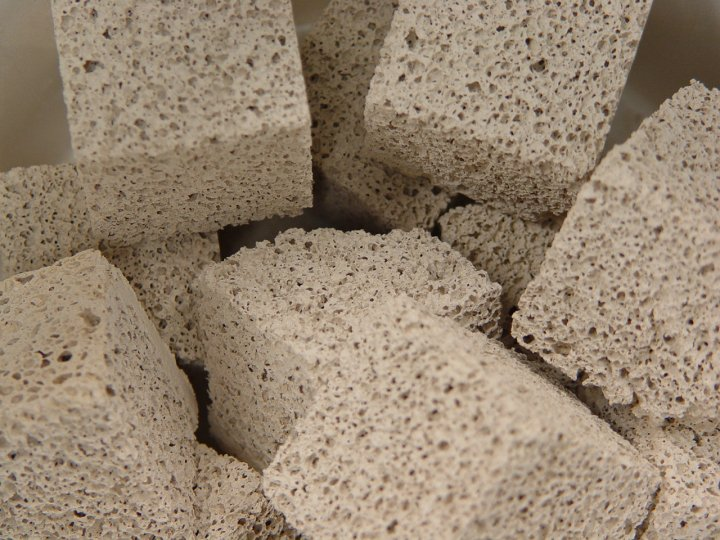
\includegraphics[width=.4\linewidth]{Porousceramic.jpg}
    \end{center}

    Now suppose we have to measure the water flow through such materials. Since
    the pores inside a porous medium are placed completely randomly. 
\end{frame}

\begin{frame}

    So in order to study such random porous objects, we need a simulation method called
    \imp{Percolation}, which gives us to build a discrete version of these materials and
    study the connnected regions inside the medium.

    \vspace{12pt}

    This model also gives us the ability to monitor the spacous parts as well. It is most
    useful for physists and applied mathematicians. It also has applications to biology,
    computer science, and social sciences.

\end{frame}

\begin{frame}
    In a percolation model, we consider an \(L\times L\) box, which we call \imp{lattice}. 

    \vspace{12pt}
    We toss a biased coin with probability \(p\) for heads and probabilty \(1-p\) for
    tails to fill some of the cells up.

    \vspace{12pt}

    So for each of the cells, we toss a coin. If the coin lands on heads, then we color
    the cell black, which means it is filled, and otherwise keep it empty.
\end{frame}

\begin{frame}

    For example, the following three \(6\times 6\) lattices are randomly filled with
    probabilities \(p=.4, .5, .6\) respectively

    \vspace{15pt}

    \begin{minipage}{.3\linewidth}
        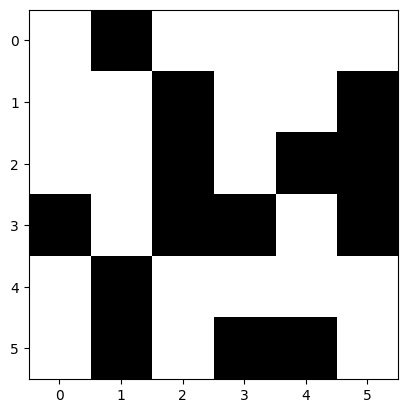
\includegraphics[width=\linewidth]{p1.png}
    \end{minipage}\hfill%
    \begin{minipage}{.3\linewidth}
        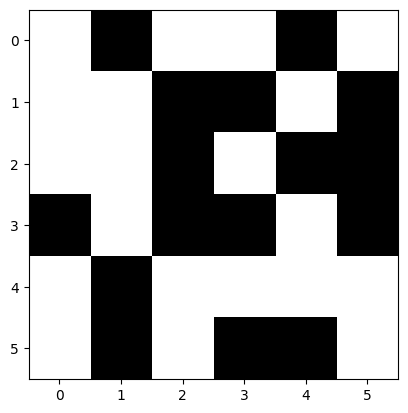
\includegraphics[width=\linewidth]{p2.png}
    \end{minipage}\hfill%
    \begin{minipage}{.3\linewidth}
        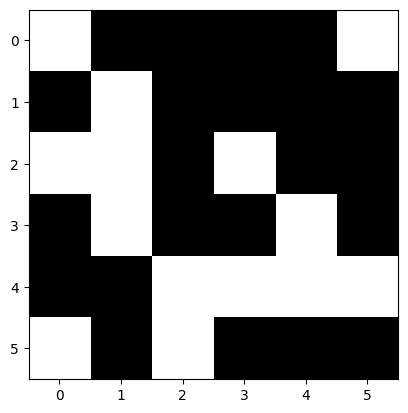
\includegraphics[width=\linewidth]{p3.png}
    \end{minipage}
\end{frame}

\begin{frame}
    \imp{Percolation is the study of connectivity.} 

    \vspace{12pt}

    In such a randomly generated lattice, we are interested in connected clusters.  A
    \imp{connected cluster} is made of some cells that are neighbor to each other and are
    all occupied. 
\end{frame}

\begin{frame}
    So in the first picture below, there are \(6\) connected clusters and there are
    \(7, \text{ and } 4\) in the second and third picture.

    \vspace{12pt}

    \begin{minipage}{.3\linewidth}
        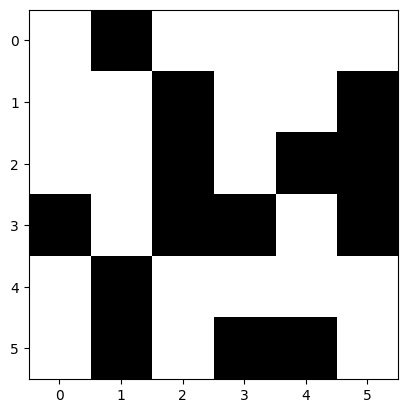
\includegraphics[width=\linewidth]{p1.png}
    \end{minipage}\hfill%
    \begin{minipage}{.3\linewidth}
        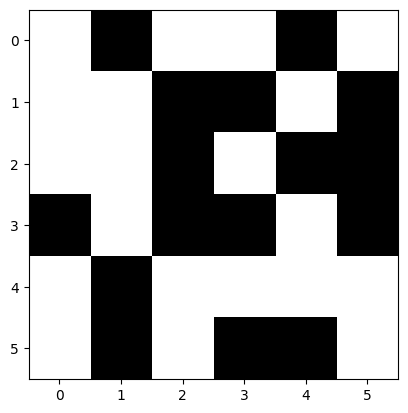
\includegraphics[width=\linewidth]{p2.png}
    \end{minipage}\hfill%
    \begin{minipage}{.3\linewidth}
        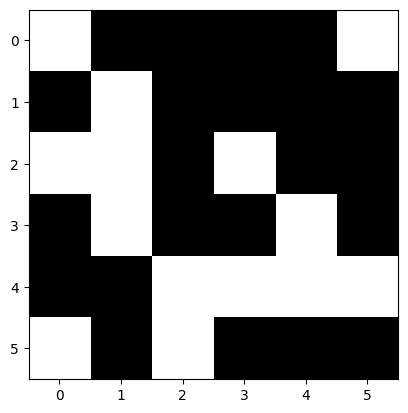
\includegraphics[width=\linewidth]{p3.png}
    \end{minipage}
\end{frame}

\begin{frame}
    
    We are even more interested in connected clusters that spans from one side of the
    lattice to the other. We call them \imp{Spanning Components}. 

    \vspace{12pt}

    We can such systems where there is a spanning cluster \imp{Percolating system}.

\end{frame}

\begin{frame} 

    \begin{minipage}{.3\linewidth}
        For example, there is no spanning cluster that goes from top to bottom of the
        lattice in the first lattice below, but there is one in the second lattice.
    \end{minipage}\hfill%
    \begin{minipage}{.3\linewidth}
        \begin{center}
            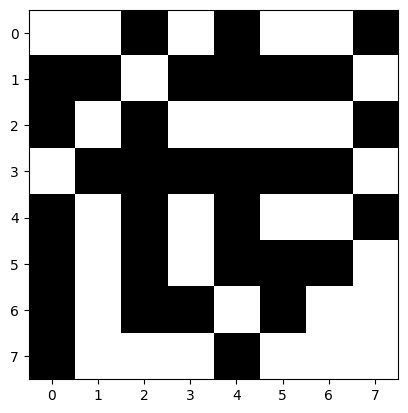
\includegraphics[width=\linewidth]{spanning1.png}
        \end{center}
    \end{minipage}\hfill%
    \begin{minipage}{.3\linewidth}
        \begin{center}
            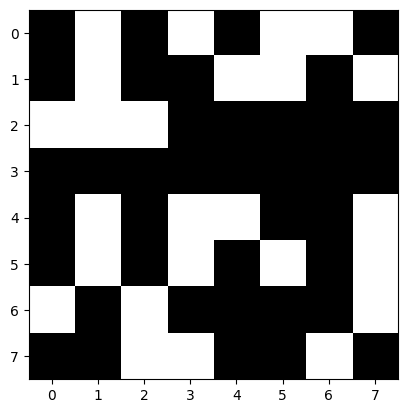
\includegraphics[width=\linewidth]{spanning2.png}
        \end{center}
    \end{minipage}

\end{frame}

\begin{frame}

    In short, we will ask this question:

    \vspace{12pt}

    \textcolor{NordOrange}{
        If we randomly generate a lattice with a biased coin with probability \(p\), for
        which values of \(0 \le p \le 1\) at system is almost certainly to be
        \textbf{Percolating}?\\
    }

    \vspace{12pt}

    \textcolor{NordOrange}{
        In other words, when will we almost certainly find a spanning connected cluster?
    }        

    \vspace{12pt}

    And in those scenarios, what happens to the connected clusters? 

\end{frame}

\begin{frame}
    \small

    Before we jump in to analyze percolation models and when such models are percolating,
    let's take a look at why do we even care about percolating theory beside studying
    porous materials.

    \begin{itemize}[left=0pt,label=\(\square\)]
        \item In situations where objects are linked to each other, and their properties
            effect others connected to them. For example in social marketing scenarios
            where buyers influence each others' preferences.
        \item In biological sciences, to predict the fragmentation of biological virus
            shells.
        \item In ecology to see how environment fragmentation impacts animal habitats.
        \item In multilayerd computer networking to find out how the layers interact with
            each other.
        \item To study traffic system in a city. Dynamic percolation models can predict
            the traffic capacity thresholds of particular junctions or roads.
        \item It has also found its application in discrete mathematics such as graph
            theory and different graph algorithms.
    \end{itemize}

    and many more...

    \normalsize
\end{frame}

\section{Taking a Closer Look}

\subsection{Basic structure}

\begin{frame}[fragile]
    So, how do we write a very basic version of this model? We want to create a lattice,
    generate a random number between \(0, 1\) for each of the cells, and check with the
    probability \(p\) if that cell should be occupied or not. The following simple code
    does such that.

    \vspace{10pt}

    \begin{lstlisting}[language=Python]
import matplotlib.pyplot as plt
import numpy.random as rnd

p = 0.5            # defining the probability here
l = rnd.rand(5, 5) # create a 8x8 array with a random probability
m = l < p          # checking if cells are occupied, true or false

plt.imshow(m, interpolation='None', cmap='binary')
plt.show()
    \end{lstlisting}
\end{frame}

\begin{frame}
    For example, one instance of this program would create the first figure shown below.
    On the second figure you can see the values of each random probability for each of the
    cells.

    \vspace{12pt}

    \begin{minipage}{.5\linewidth}
        \begin{center}
            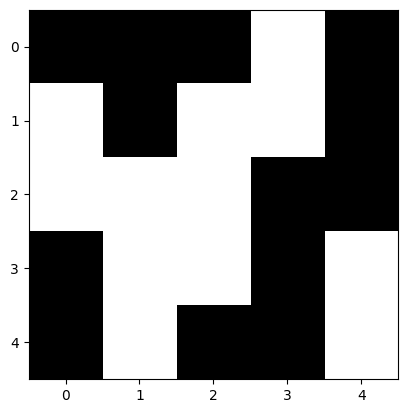
\includegraphics[width=.7\linewidth]{random_array_true-false.png}
        \end{center}
    \end{minipage}\hfill%
    \begin{minipage}{.5\linewidth}
        \begin{center}
            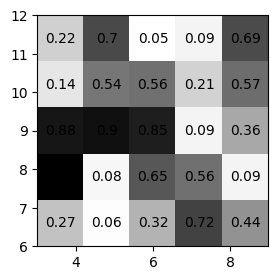
\includegraphics[width=.74\linewidth]{random_array.png}
        \end{center}
    \end{minipage}
\end{frame}

\begin{frame}[fragile]
    Now since we are interested about the \imp{clusters}, we can have them in different
    shades to be like:

    \begin{minipage}{.63\linewidth}
        \begin{lstlisting}[language=python]
from scipy.ndimage import measurements
from random import shuffle

lw, num = measurements.label(m)
b = np.arange(lw.max() + 1)
shuffle(b[1:])
shuffledLw = b[lw]
        \end{lstlisting}
    \end{minipage}\hfill%
    \begin{minipage}{.35\linewidth}
        \begin{center}
        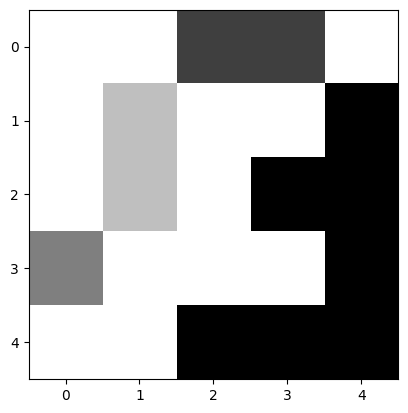
\includegraphics[width=\linewidth]{cluster.png}
        \end{center}
    \end{minipage}

\end{frame}

\subsection{Defining Percolation Threshold}

\begin{frame}
    We previously said that we will be interested at when we have a spanning cluster. To
    get a better understanding, we define the following:

    \vspace{12pt}

    \imp{\textbf{Percolation Threshold:}} \textcolor{NordOrange}{The smallest probability
    \(p\) for which any randomly generated lattice of a fixed size with probability \(p\)
    is almost certain to have a spanning cluster.}

\end{frame}

\begin{frame}
    For example, the percolation threshold for a 2D infinite lattice is \(0.593\) meaning
    that if we color the cells of an infinite 2D lattice with the probability \(p=0.593\),
    then there will be certainly a cluster that spans from negative infinity to positive
    infinity.
\end{frame}

\begin{frame}
    Now the natural question is, why is the threshold so important?

    \vspace{12pt}

    Say we have a random situation, where our product quality has to be a certain level to
    reach the most number of customers. Now we want to minimize the cost. So if we
    consider the situation to be a percolation model, our quality should be somewhere
    close to the percolation threshold.
\end{frame}

\subsection{Finding the Percolation Threshold}

\begin{frame}[fragile]
    Now, how do we find the percolation threshold for a given lattice of size \(L\times
    L\)? 
    \vspace{12pt}

    Previously where we used \texttt{lw, num = measurements.label(m)}, we named the
    clusters by numbers. For example, this like would turn the left \texttt{nparray} to
    the right \texttt{nparray}.

    \vspace{10pt}

    \begin{minipage}{.6\linewidth}
\begin{lstlisting}
[[ True  True False  True False]
 [ True False  True  True False]
 [False  True False False False]
 [ True  True False  True False]
 [ True False False  True False]]
\end{lstlisting}
    \end{minipage}\hfill%
    \begin{minipage}{.3\linewidth}
\begin{lstlisting}
[[1 1 0 2 0]
 [1 0 2 2 0]
 [0 3 0 0 0]
 [3 3 0 4 0]
 [3 0 0 4 0]]
\end{lstlisting}
    \end{minipage}
\end{frame}

\begin{frame}
    So if a spanning cluster existed, then the leftmost column and the rightmost column
    would have one number in common, which would mean that there were a cluster that
    spanned from the left border to the rightmost border.
\end{frame}

\begin{frame}[fragile]
    To find the percolation threshold, we divide the interval \([0, 1]\) into 100 or more
    equally spaced points. And then run the simulation to randomly generate lattices and
    check if there is spanning cluster in that lattice. The pseudocode is given below:

    \begin{lstlisting}
arr = np.linspace(0, 1, 100)
for p in arr:
    samples = produce_samples(p)
    if check_if_spanning_cluster_exists(samples):
        return p
    \end{lstlisting}

    This will find the smallest value of \(p\) for which almost certainly random lattices
    will be percolating.
\end{frame}

\end{document}
